\graphicspath{{RL/fig}}
\chapter{Reinforcement Learning}
\label{chap:RL}

\section{Introduction}
In previous chapters we discussed methods which required knowledge about the model of the environment. This knowledge was embedded in the probability transition matrix P. Often times it is not possible to know the model of the environment beforehand. We therefore in this chapter look at methods which do not require models.
This chapter is divided into two sections:
\begin{itemize}
	\item Model-free prediction which \textbf{estimates}, by \textit{evaluating}, the value function of an MDP. 
	\item Model-free control which \textbf{optimizes} the value function of an MDP.
\end{itemize}

\section{Model-free prediction}
\subsection{Monte Carlo background}
Sutton and Barto claims that, the term Monte Carlo is generally used for
any estimation technique where a large portion of its operation is random \cite{sutton_barto}. In this chapter we used the term specifically for methods based on averaging returns.
Sutton and Barto continues describing Monte Carlo methods as solving reinforcement learning problems by averaging sample returns \cite{sutton_barto}.
Monte-Carlo methods require only experience, which it obtains by sampling sequences of states, actions and rewards. By sampling enough times,by the law of large numbers, eventually we will obtain an accurate model of the environment being sampled from \cite{sutton_barto}.
\subsection{Monte Carlo prediction}
Monte-Carlo policy evaluation works as follows. We define a total return S in state s as S(s) and a integer counter N(s), with both S(s) and N(s) initialized to zero. 
Then at time step t and state s we increment a running counter N(s) = N(s)+1. This can be done in two ways, one being only incrementing N(s) the \textit{first} time state s is reached, the other being incrementing N(s) \textit{every} time states s is reached \cite{David_Silver}.

In this chapter we use the method of incrementing the counter every instance that state s is seen.
Then we increment the total reward S(s) =  S(s) + $G_t$.
Finally we calculate the value function $V(s)=\frac{S(s)}{N(s)}$.
Then V(s) $\to V_\pi(s)$ as N(s) $\to \infty$.

In order to incrementally do Monte-Carlo updates, David Silver introduces the concept of an incremental mean $u_k$ in \cite{David_Silver}. The derivation for $u_k$ from a standard mean is as follows:
\begin{align}
	u_k &= \frac{1}{k}\sum_{j=1}^{k}x_j\\
	&= \frac{1}{k}(x_k + \sum_{j=1}^{k-1}x_j) \nonumber\\
	&= \frac{1}{k}(x_k +(k-1)u_{k-1})\nonumber\\
	&= u_{k-1} + \frac{1}{k}(x_k - u_{k-1}).
	\label{eq:u_k}
\end{align}
The variable that we are averaging over is V(s), hence $u_{k-1}=V(s)$. The counter $N(s)=t=k$ and return $G_t =x_k$ in equation \ref{eq:u_k}. Substituting these variables into equation \ref{eq:u_k} yields:

\begin{align}
	N(S_t) &= N(S_t) + 1 \\
	V(S_t) &= V(S_t) + \frac{1}{N(S_t)}(G_t - V(S_t)).
\end{align}
David Silver claims that it can be useful to disregard the running counter and instead make $\frac{1}{N(S_t)}$ a constant $\alpha$ as follows:
\begin{equation}
	V(S_t) = V(S_t) + \alpha(G_t - V(S_t)).
	\label{eq:monte_carlo}
\end{equation}
Equation \ref{eq:monte_carlo} gives us a way to find the optimal policy $V_\pi(S_t)$ by iteratively updating $V(S_t)$.
\subsection{Temporal Difference (TD) Learning}
Temporal difference (TD) learning uses a combination of Monte Carlo an dynamic programming (DP) ideas. TD is one of the unique aspects of reinforcement learning, unlike Monte Carlo and DP which have more general applications besides reinforcement learning \cite{sutton_barto}. Like Monte Carlo TD learns without requiring a model of the environment. Because TD is a reinforcement method, it can be split into prediction and control methods as was stated in the introduction of this chapter. Here in this section we only describe the prediction method, while the next section will discuss two control methods, namely SARSA and Q-learning.\\
The aim of TD learning is to learn a value function $v_\pi$ from experience by following policy $\pi$. 
The simplest form of TD is replacing the return $G_t$ in equation \ref{eq:monte_carlo} from the previous section as follows:
\begin{equation}
	V(S_t) = V(S_t) + \alpha({\color{red}R_{t+1} +  \gamma V(S_{t+1})} - V(S_t)).
	\label{eq:monte_carlo_TD}
\end{equation}
Where $[{\color{red}R_{t+1} +  \gamma V(S_{t+1})}]$ is known as the TD target, the value which $V(S_t)$ tends to as $t \to \infty$ and
$[{\color{red}R_{t+1} +  \gamma V(S_{t+1})} - V(S_t)]$ is known as the TD error. The aim of TD learning is to reduce the TD error to zero and update $V(S_t)$ to the estimated return ${\color{red}R_{t+1} +  \gamma V(S_{t+1})}$.
Suttton and Barto mathematically describes the relationship between MC and TD using what they define as the n-step return $G_{t}^{(n)}$ described by:
\begin{equation}
	G_{t}^{(n)} = R_{t+1} + \gamma R_{t+2} + ... + \gamma^{n-1}R_{t+n} + \gamma^{n}V(S_{t+1}).
\end{equation}
For clarity we show 
$G_{t}^{(n)}$ for a few values of n as follows:\\
\begin{align}
	 {\color{red}(TD)} n &= 1: G_{t}^{(1)} = R_{t+1}+\gamma V(S_{t+1}) \label{eq:td} \\
	n &= 2 : G_{t}^{(2)} = R_{t+1}+ \gamma R_{t+2}+\gamma^2 V(S_{t+2}) \\
	{\color{red}(MC)} n &= \infty : G_{t}^{(\infty)} = R_{t+1}+ \gamma R_{t+2}+...+\gamma^{T-1} R_T. \label{eq:mc_td}
\end{align}
What can be seen is, as n $\to$ $\infty$, the return in TD learning turns into the same form as in Monte Carlo. Hence Monte Carlo can be said to be a special case of TD learning.
Similarly Sutton and Barto describes n-step TD as:
\begin{equation}
	V(S_t) = V(S_t) + \alpha(G_t^{(n)} - V(S_t)).
	\label{eq:n_step_TD}
\end{equation} 
What we now have is a method to control how many steps we want an agent to look ahead. This is useful because $V(S_t)$ can converge more quickly to $V_\pi(S_t)$, if n is adjusted accordingly. Normally one has to test for different values of n to see which value works best for the specific problem at hand. When comparing Monte Carlo methods which has to wait for the entire episode of states to play out with TD, TD works much better in applications where waiting for an entire episode to complete might be too slow \cite{sutton_barto}. Also some applications have no episodes at all, as the sequence of states can continue indefinitely \cite{sutton_barto}. Sutton and Barto state that it has not been mathematically proven yet that TD converges faster that Monte Carlo methods, but that in practice TD converges faster on stochastic tasks \cite{sutton_barto}. In the next section we no longer look at estimating the state-value function $V_\pi(S_t)$, but instead deal with \textit{state-action} pairs in order to find the optimal policy $\pi_{*}$.

\section{Model-free control}
There are two ways that model-free control can be implemented:

\textbf{On-policy learning:}
Learning characteristics of a policy $\pi$ by sampling from $\pi$

\textbf{Off-policy learning:}
Learn characteristics of policy $\pi$ by sampling another policy

\noindent Previously, when using greedy policy improvement over the value function V(s) we had in equation \ref{pi'}:
\[\pi^{'}(s) = \max\limits_{a \in A}(R^{a}_s+\gamma\sum_{s'\in S}P^{a}_{ss'}v_*(s'))\]
If we now instead apply greedy policy improvement over the state action function Q(s,a) we have that:
\begin{equation}
	\pi^{'}(s) = \max\limits_{a \in A}Q(s,a).
	\label{eq:pi'}
\end{equation}
Which means that we now maximize not only across the state space as in equation \ref{pi'}, but rather the entire state-action space when using model-free policy iteration. One should notice that to find the optimal policy we no longer need a model of the environment. In other words there is no dependency on the probability matrix $P^{a}_{ss'}$ seen in equation \ref{eq:pi'}.

However there now arises a problem when always having the agent act greedily. Which is that the agent will take the action which looks best looking only one step ahead, while another action might have been better in the long term. To overcome this limitation Sutton and Barto introduces the topic of $\epsilon$-Greedy exploration \cite{sutton_barto}.

To ensure that the agent explores occasionally instead of always taking the greedy action, we let the agent act randomly with a probability $\epsilon$. This can mathematically be expressed as:
\begin{align}
	\pi(a|s)=\begin{cases}
		\frac{\epsilon}{m}+1, & \text{if $a^* = \argmax\limits_{a \in A}Q (s,a)$}\\
		\frac{\epsilon}{m}, & \text{otherwise}
	\end{cases}
	\label{eq:pi_epsilon-greedy}
\end{align}
This results in the agent exploring occasionally and perhaps finding other policies which are even better than the one which it is following. The value of $\epsilon$ is an hyper parameter, that is tweaked according to the specific application. Usually an $\epsilon$ os 10\% is a good starting value.
\\
{\color{red} \huge place monte-carlo control here possibly...}
\subsection{SARSA}
\begin{figure}[!htb]
	\begin{subfigure}{.5\textwidth}
		\centering
		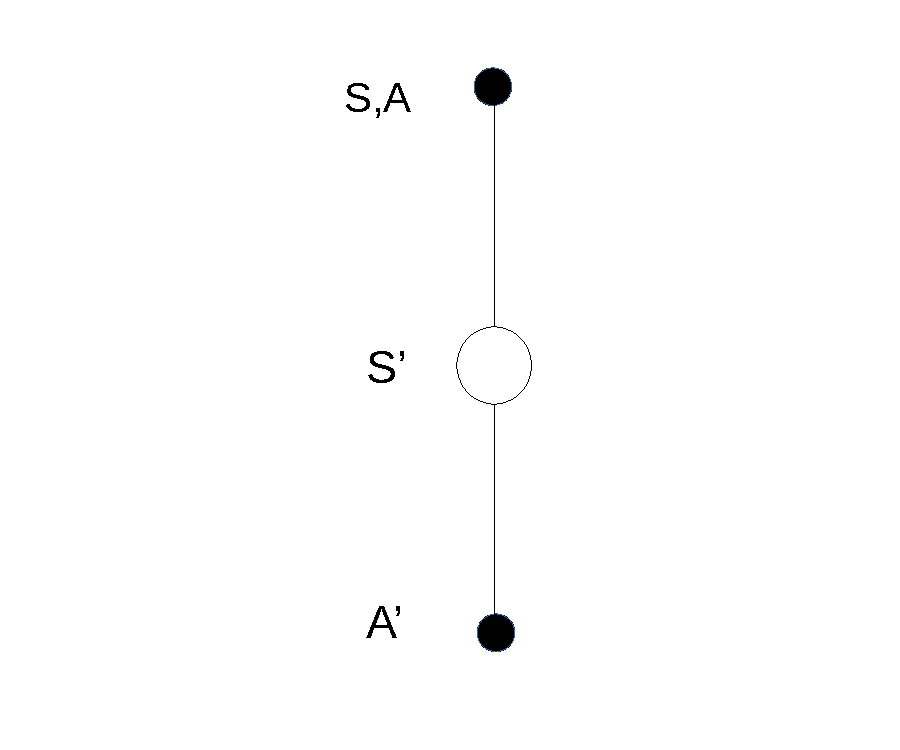
\includegraphics[width=1\linewidth]{RL/fig/sarsa_state_diagram.pdf}
		\caption{SARSA state diagram representation\cite{David_Silver}}
		\label{fig:sarsa_state_diagram}
	\end{subfigure}
	\begin{subfigure}{.49\textwidth}
		\centering
		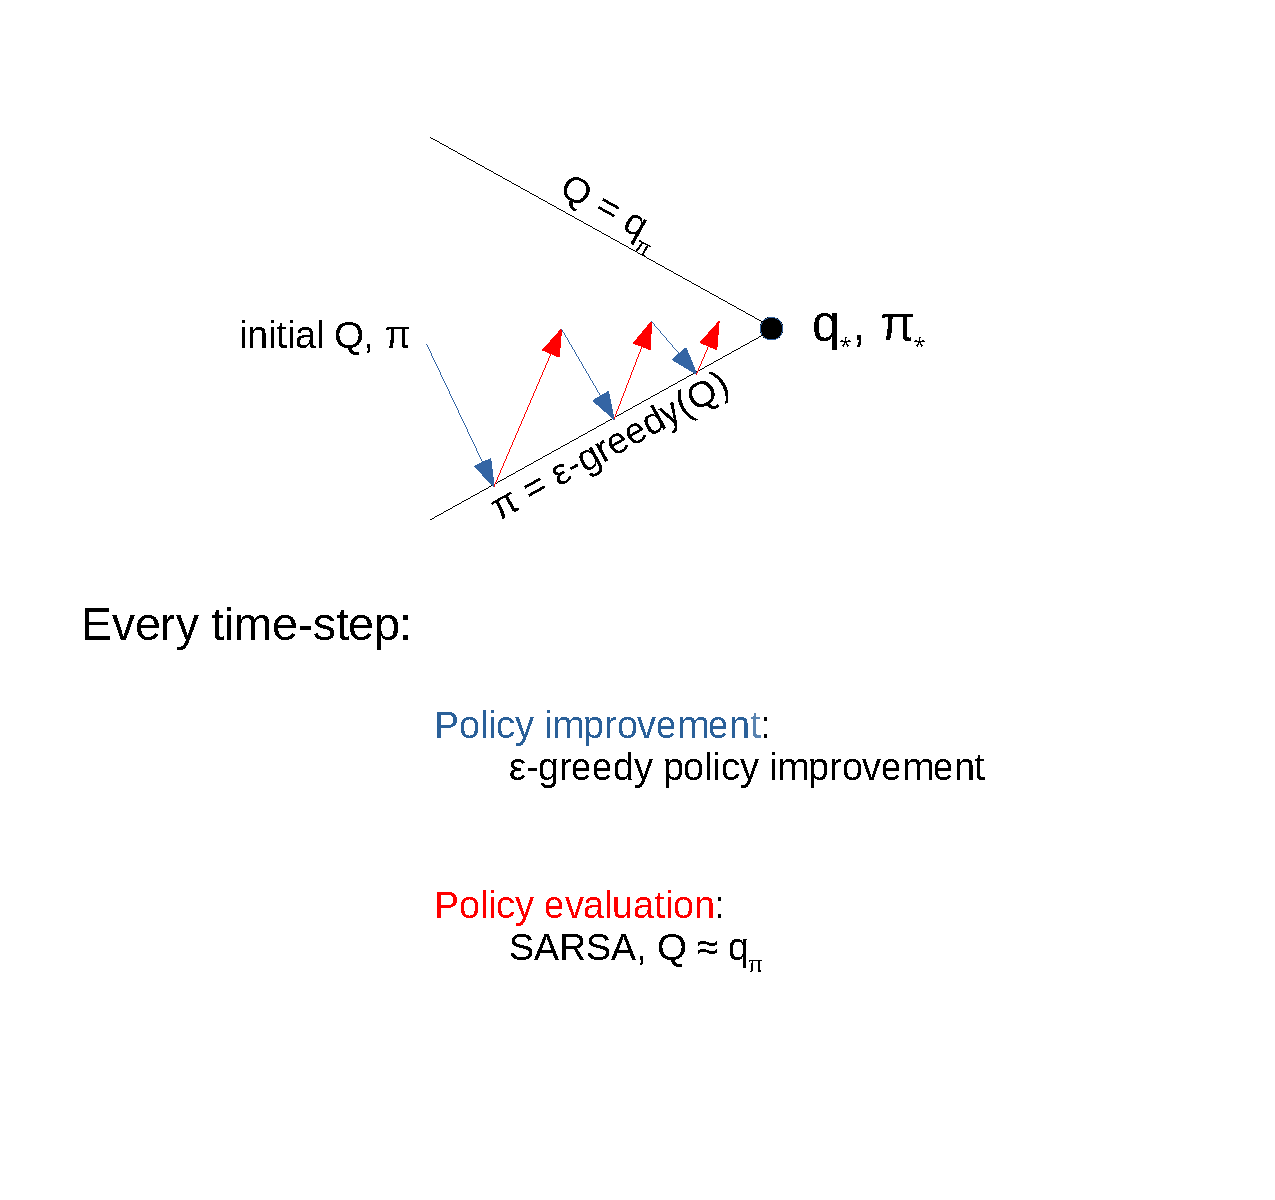
\includegraphics[width=1\linewidth]{RL/fig/sarsa_on_policy_control.pdf}
		\caption{SARSA on policy control diagram\cite{David_Silver}}
		\label{fig:sarsa_on_policy}
	\end{subfigure}
	\begin{subfigure}{1\textwidth}
		\centering
		\includegraphics[width=1\linewidth]{RL/fig/sarsa_algorithm.jpeg}
		\caption{SARSA algorithm\cite{David_Silver}}
		\label{fig:sarsa_algorithm}
	\end{subfigure}
	\caption{SARSA diagrams \cite{David_Silver}}
	\label{fig:sarsa}	
\end{figure}
In Figure \ref{fig:sarsa_state_diagram} the concept of the State-Action-Reward-State-Action (SARSA) learning method is graphically shown. For every state action pair, we can calculate the q-function using the same concept as TD learning as follows:

\begin{equation}
	Q(S,A) = Q(S,A) + \alpha[R+\gamma Q(S',A') - Q(S,A)]
	\label{eq:sarsa_update}
\end{equation}
Where $R+\gamma Q(S',A')$ is the TD target. In Figure \ref{fig:sarsa_on_policy} we see that the way SARSA learns the optimal policy $\pi_{*}$ is not by completely following policy $\pi$. But instead by stopping somewhere in between which can be seen by the arrows stopping in the middle of the two lines for Q and $\pi$. If Monte Carlo was instead used to learn the optimal policy $\pi_{*}$ we would have a diagram similar to \ref{fig:greedy_policy_iteration}, where the entire episode has to play out before the algorithm updates.
We can also define n-step Q-return:
\begin{equation}
	q_{t}^{(n)} = R_{t+1} + \gamma R_{t+2} +...+ \gamma^{n-1}R_{t+n}+\gamma^{n}Q(S_{t+n})
	\label{eq:q_return}
\end{equation}
The goal of n-step SARSA is to update Q(s,a) towards the n-step Q-return $q_t^{(n)}$.
\begin{equation}
	Q(S_t,A_t) = Q(S_t,A_t) + \alpha[q_{t}^{(n)} - Q(S_t,A_t)]
	\label{eq:sarsa_n_step}
\end{equation}
When we have n = 1 then we have SARSA updates and at n = $\infty$ we have Monte Carlo updates. All values of n $\in [1,\infty]$ is between SARSA and Monte Carlo.
Figure \ref{fig:sarsa_algorithm} shows the algorithm that can be used to implement SARSA. Later in chapter \ref{chap:Experiments_and_Results} we will implement this algorithm which will make the concept clearer.
\subsection{Q-learning}
\begin{figure}[!htb]
	\begin{subfigure}{0.5\textwidth}
		\centering
		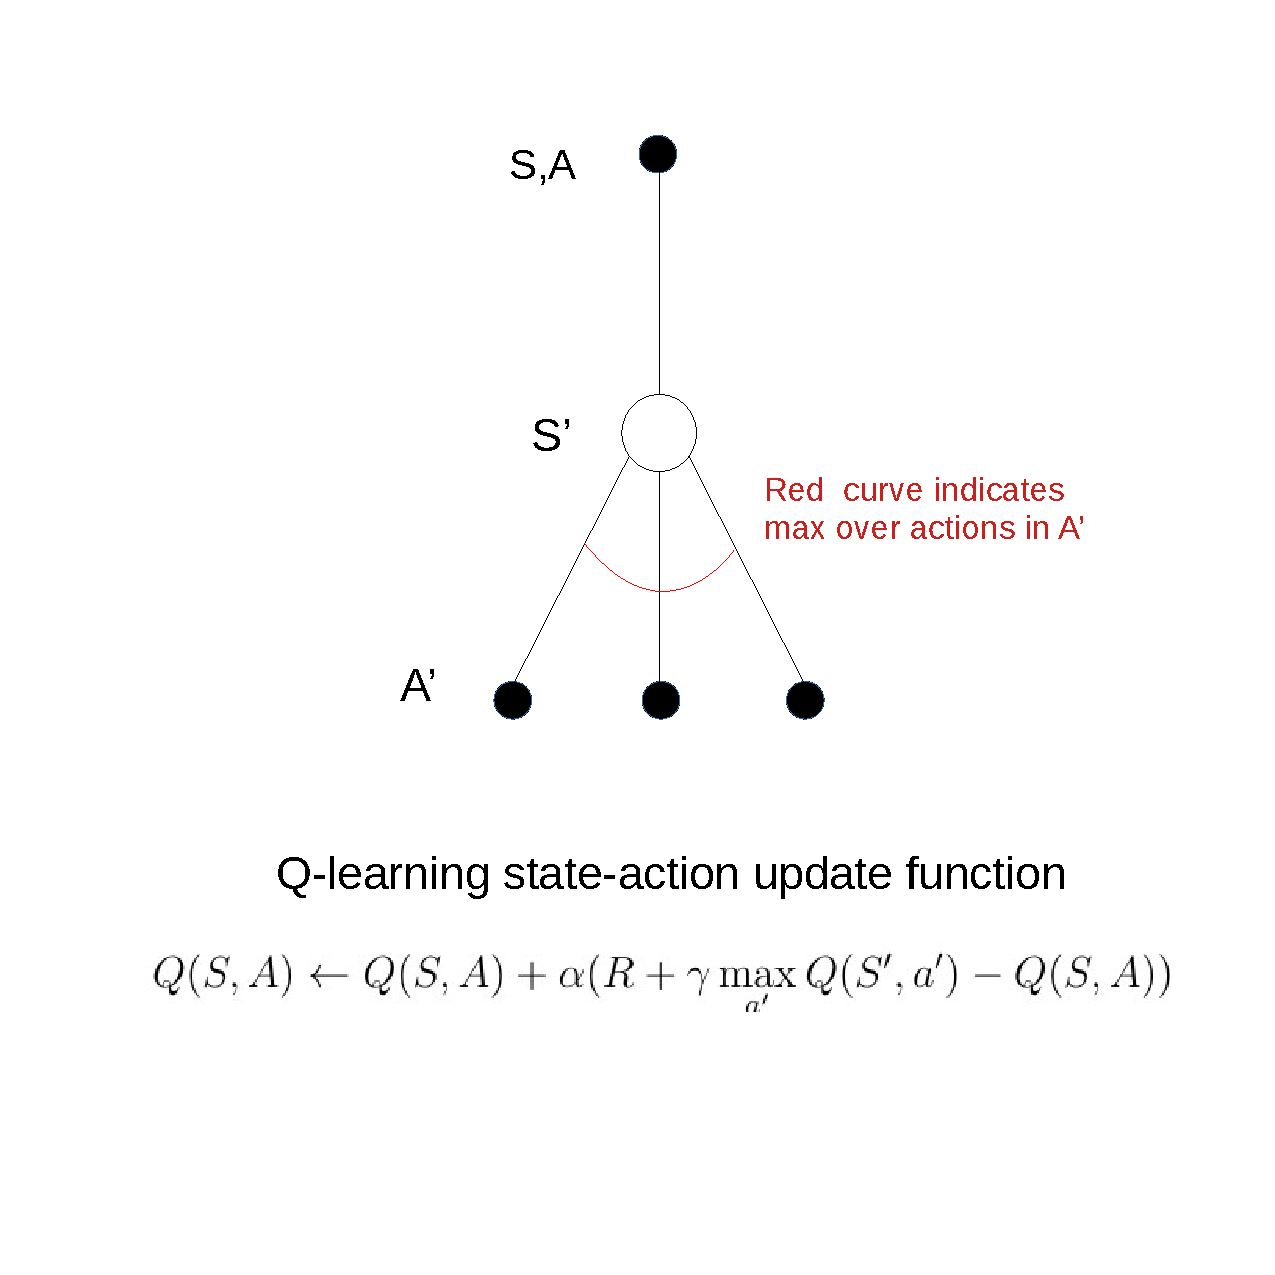
\includegraphics[width=1\linewidth]{RL/fig/q_learning_state_diagram.pdf}
		\caption{Q-learning state action diagram\cite{David_Silver}}
		\label{fig:q_learning_state_action_diagram}
	\end{subfigure}
	\begin{subfigure}{0.5\textwidth}
		\centering
		\includegraphics[width=1\linewidth]{RL/fig/q_learning_algorithm.png}
		\caption{Q-learning algorithm\cite{David_Silver}}
		\label{fig:q_learning_algorithm}
	\end{subfigure}
	\caption{Q-learning state-action diagram and algorithm}
	\label{Q-learning}
\end{figure}
\begin{equation}
	Q(S,A) \leftarrow Q(S,A) + \alpha(R + \gamma\max\limits_{a'}Q(S',a') - Q(S,A))
	\label{eq:q_learning_update_function}
\end{equation}
What we have been dealing with up to now in this chapter dealt with on-policy learning.
We describe now Q-learning which falls under off policy learning. By comparing Figure \ref{fig:q_learning_state_action_diagram} and Figure \ref{fig:sarsa_state_diagram}, we can see that the only difference between Q-learning and SARSA is that Q-learning takes the maximum action A', instead of a singular determined A', which results in the maximum Q-return. Where the Q-return was earlier defined in equation \ref{eq:q_return}.
Hence in equation \ref{eq:q_learning_update_function} we see the Q-learning update function is very similar to the SARSA function in equation \ref{eq:sarsa_update}.
Q-learning control always converges to the optimal action value function meaning, $Q(S,A) \to q_*(S,A)$. 
